\section{Seleção}
O algoritmo Seleção é um método de ordenação instável, como mostra a figura \ref{fig:selecao}. A ideia é bastante simples: execute $n$ iterações; na i-ésima iteração, selecione o i-ésimo menor elemento e coloque-o na posição $i - 1$. Uma propriedade interessante desse algoritmo é que ele realiza o número mínimo possível de trocas para ordenar o vetor.

\lstinputlisting[language=C]{codigos/inf/3_selecao.txt}

\begin{figure}[H]
\Caption{\label{fig:selecao}Seleção aplicado ao vetor \([3, 3, 2, 5]\).}
\centering
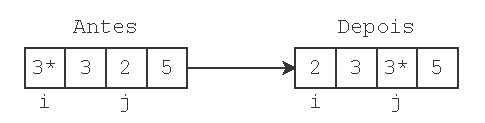
\includegraphics[scale=1.0]{figuras/pdf/selecao.pdf}
\Fonte{Elaborado pelo autor}
\end{figure}

\subsection*{Corretude}
É invariante que, ao final de cada iteração do laço externo, os elementos de $v[0..i]$ já estejam em suas posições definitivas. Portanto, ao final da última iteração, quando $i$ for igual a $n - 1$, o vetor $v[0..n - 1]$ estará ordenado.

\subsection*{Desempenho}
O ponto crítico do algoritmo Seleção é o teste condicional \textit{if} na linha 5. A quantidade de vezes que esse ponto é executado é sempre dada pela soma \ref{eq:1}, ou seja, não há melhor nem pior caso. Portanto, esse algoritmo sempre requer tempo igual a $\Theta(n^2)$.
